\section{Mesh}
Un \eng{mesh} n'est en réalité qu'un ensemble de triangle, de texture et de
coordonnées de textures. Ce n'est donc pas dans l'agrégation que se situe la
difficulté.\\

Le vrai problème se trouve dans le nombre de triangles qu'un mesh peut
contenir. Sans structure accélératrice, le calcul de chaque pixel devrait
tester l'intersection avec tout les triangles. C'est inimaginable et le temps
de la calcul serait multiplié par le nombre de triangles de la scène (certains
de mes modèles possèdent plus de 80 000 faces).

\subsection{L'\tsl{octree}}
Pour optimiser les calculs d'intersection, j'ai décidé d'utiliser une structure
appelée \tsl{Octree}. Cette structure permet de diviser l'espace et de le
représenter par un arbre. Son fonctionnement est relativement simple :
\begin{description}
  \item [\tbf{Initialisation}] Lors de la création, trouver le cube englobant
    tous les triangles du \eng{mesh}. Puis, récursivement, diviser ce cube en
    8 cubes (au maximum), chacun moitié du cube existant. Continuer tant que
    le contenu du cube courant est supérieur au contenu maximal. Après cette
    étape, nous nous retrouvons avec une subdivision du type de celle
    représenté à la \tsl{fig. \ref{octree}}.
  \item [\tbf{Calcul d'intersection}] D'abord, vérifier que le rayon
    intersecte le cube englobant. Puis, pour chacun de ses cubes enfant,
    établir la collision.\footnote{Il est possible d'accélérer le résultat en
    tenant compte de la direction du rayon sortant lors de l'intersection avec
    un cube.} Prendre le plus prêt et descendre comme ceci jusqu'à
    un cube feuille. Enfin tester l'intersection avec les triangle de la
    feuille.
\end{description}

\begin{figure}[h]
  \begin{center}
   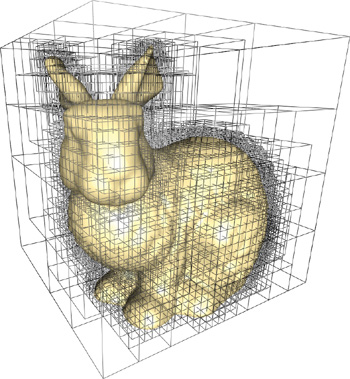
\includegraphics[width=.5\textwidth, keepaspectratio=true]{img/octree}
   \caption{Un \tsl{octree}\ construit sur le lapin de
   Standford\label{fig:octree}. On observe que les zones denses en triangles
   sont plus subdivisées que les autres zones contenant de moins de
   polygones.}
  \end{center}
\end{figure}

Il devient alors évident que le nombre de tests d'intersection est
considérablement réduit.

En effet, quelques calculs d'intersections très simples (avec des boites
alignées aux axes ---
AABB\footnote{\url{http://www.cgal.org/Manual/latest/doc_html/cgal_manual/AABB_tree/Chapter_main.html}})
suffisent à atteindre une feuille et par conséquent à tester aux maximum une
centaine d'intersections avec des triangles.

\subsection{Exemple}
\begin{figure}[h]
  \begin{center}
    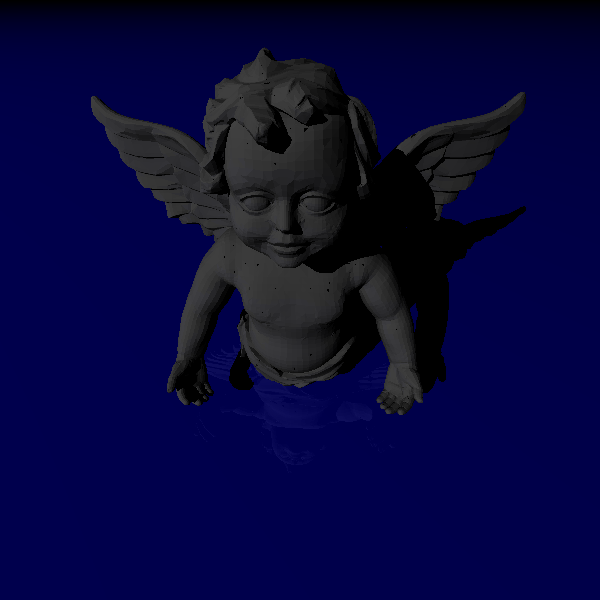
\includegraphics[width=1\textwidth, keepaspectratio=true]{../../diary/15.png}
    \caption{Un exemple de rendu de mesh (+80 000 faces, $<$ 1 minutes)\label{fig:angel}}
  \end{center}
\end{figure}

\subsection{Amélioration}
Aucune.

\subsection{Bug connu}
\begin{description}
  \item [Problème d'appartenance des triangles :] Après un débugage pourtant
    poussé, je n'ai pas réussi à comprendre pourquoi certains triangles
    n'était jamais ajouté à la structure. Ce n'est pourtant pas des triangles
    proches de la \tsl{bounding box}. Ce problème est observable sur la
    \tsl{fig. \ref{fig:angel}}.
\end{description}
